\documentclass[a4paper,12pt]{article}
\usepackage[utf8]{inputenc}
\usepackage{graphicx}
\usepackage{geometry}
\usepackage{titlesec}
\usepackage{enumitem}
\usepackage{xcolor}

% Mise en page
\geometry{top=1in, bottom=1in, left=1in, right=1in}

% Format des sections
\titleformat{\section}{\large\bfseries\sffamily}{}{1em}{}
\titleformat{\subsection}{\normalsize\bfseries\sffamily}{}{1em}{}

% Suppression de la numérotation des sections
\setcounter{secnumdepth}{0}

\begin{document}

% Photo de profil
\begin{minipage}{0.3\textwidth}
    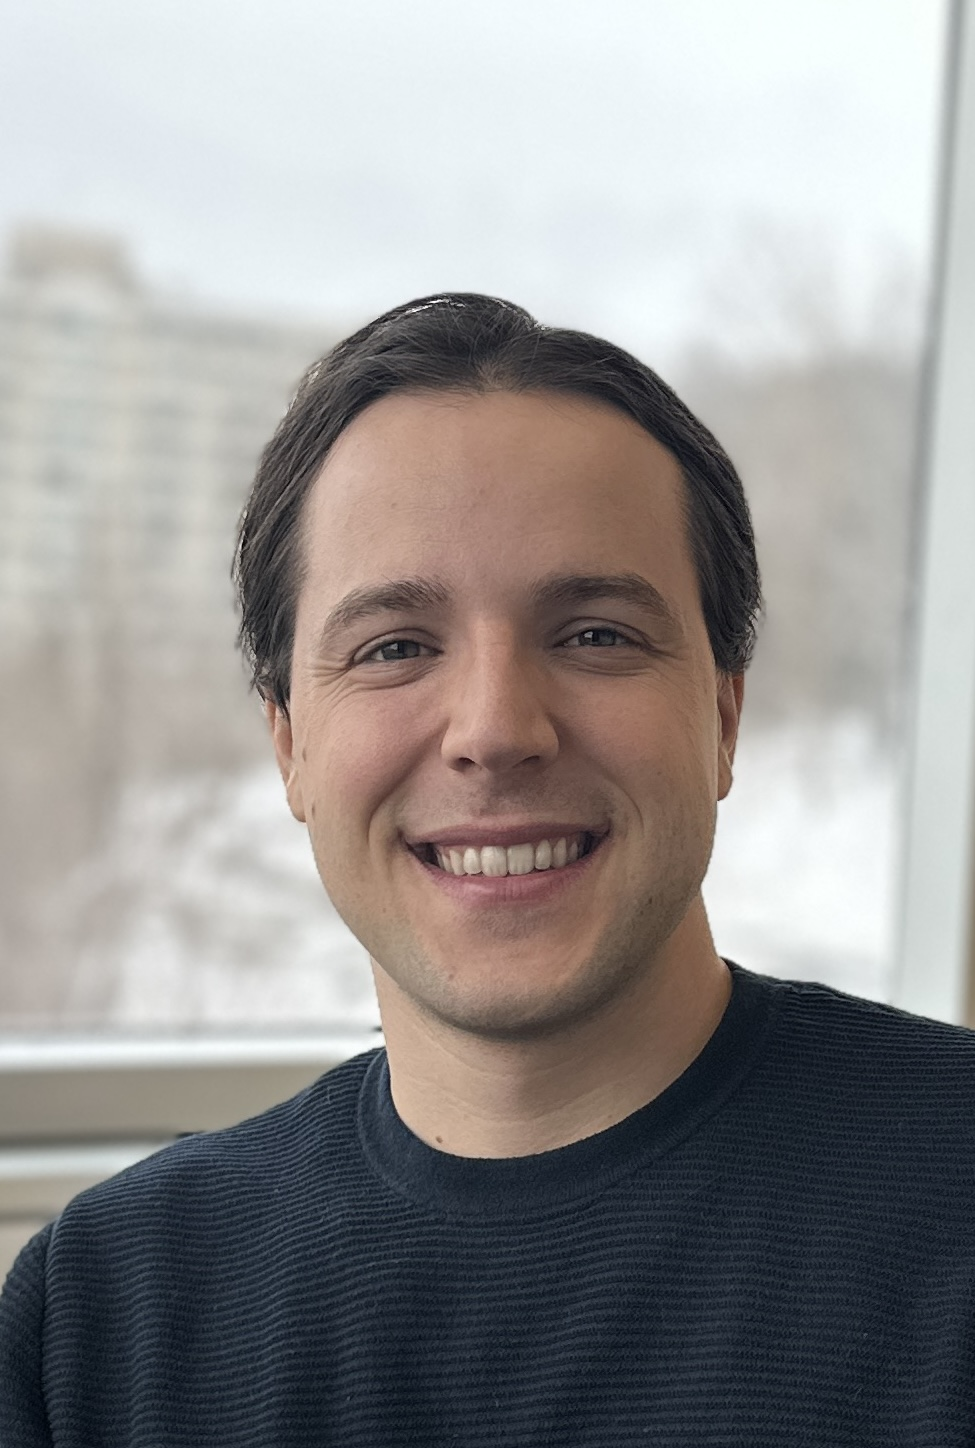
\includegraphics[width=0.5\textwidth]{../images/profile.jpg} % Remplacez par le chemin de votre photo
\end{minipage}
\begin{minipage}{0.65\textwidth}

% Nom et titre
    {\LARGE \textbf{Pierre-Yves Lajoie}
    \vspace{0.5em}}\\
    \vspace{0.5em}
    {\large Professeur adjoint en Robotique et IA}\\
    \vspace{0.2em}
    \vspace{0.2em}
    pierre-yves.lajoie@polymtl.ca\\
    \vspace{0.5em}
    https://lajoiepy.github.io/\\
\end{minipage}
\vspace{1em}

% Biographie
\section{Biographie}
Je suis professeur adjoint en robotique et intelligence artificielle au département de génie informatique et génie logiciel à \textbf{Polytechnique Montréal}. 

Avant de devenir professeur, j'ai complété un doctorat à Polytechnique, durant lequel j'ai été chercheur visiteur au \textbf{Mobile Robotics Group de l'Université d'Oxford} et au \textbf{SPARK Lab du Massachusetts Institute of Technology (MIT)}, ainsi que chez \textbf{Samsung Research America}.

Mes recherches portent sur la robotique autonome, avec un accent sur la perception 3D, la vision par ordinateur, les systèmes distribués et l'intelligence artificielle appliquée aux systèmes multi-robots.

% Intérêts de recherche
\section{Intérêts de recherche}
\begin{itemize}[leftmargin=1em]
    \item Intelligence spatiale
    \item Apprentissage machine pour la robotique
    \item Fusion de capteurs et localisation (SLAM) dans des environnements complexes
    \item Planification et coordination d'équipes robotiques autonomes
    \item Applications en robotique spatiale, fabrication automatisée et robotique de service
\end{itemize}

% Étudiants potentiels
\section{Étudiant·es potentiel·les}  
Je suis à la recherche d’étudiant·es motivé·es et curieux·ses, ayant une solide formation en programmation, en intelligence artificielle et/ou en robotique, pour travailler sur la compréhension de scène, la perception et l’apprentissage en robotique autonome dans des environnements incertains.


\vspace{2em}
\textbf{Si vous êtes intéressé(e) à travailler avec moi, pour un stage/maîtrise/doctorat veuillez m'envoyer votre CV, relevé de notes et un court résumé de vos intérêts de recherche.}

\vspace{1em}
\noindent N’hésitez pas non plus à m’écrire si vous êtes simplement curieux·se et que vous souhaitez en savoir plus.

\vspace{1em}
Adresse courriel: pierre-yves.lajoie@polymtl.ca

\end{document}
